\documentclass[10pt]{article}

\usepackage{geometry}
\usepackage{graphicx}

\graphicspath{ {Diagram/} }
\geometry{verbose,tmargin=1.5cm,bmargin=1.5cm,lmargin=1.5cm,rmargin=1.5cm,headheight=1cm,headsep=1cm,footskip=1cm}

\begin{document}
\title{Lightweight publish-subscribe application protocol}
\author{Luca Fochetta, Andrea Martino}

\maketitle


\section{Introduction}
In this document we will try to summarise how we implemented a lightweight version of \emph{MQTT} on \emph{TinyOS} running on \emph{TelosB} motes. We have extensively tested our implementation in a simulated environment provided by \emph{Cooja}. You can find the complete implementation on \emph{https://github.com/fochetz/IoTProject2017}.

\section{Modules}

\subsection{Common}
We have two components that are in common between the \emph{PanC} and the \emph{Client}:
\begin{itemize}
\item \textbf{QueueSenderC}: a special sender that receives a generic message, inserts in a queue and then sends it. If the packet is not acknowledge it is reinserted in the queue tail. The component will periodically try to send the first packet in the queue. \emph{QueueSender} can potentially be used by any components that needs to reliably send a message.
\item \textbf{PublishModuleC}: This module sends the publish message(using the \emph{QueueSender}) and signals trough an event whenever a publish message is received.
\end{itemize}

\subsection{Client}
\emph{Client} is built upon a main module, \textbf{ClientC} that uses the two common components and the following ones:
\begin{itemize}
\item \textbf{ConnectionModuleC}: sends \emph{CONNECT} message to the \emph{PanC} and receives \emph {CONNACK} message. When received, it signals an event to the \emph{Client} main component.
\item \textbf{SubscribeModuleC}: sends \emph{SUBSCRIBE} message (if the node wants to subscribe to some topic) and receives \emph{SUBACK} message. When received, it signals an event to the \emph{Client} main component.
\item \textbf{FakeSensorP}: simulates different sensors and signals when a specific sensor is read to the \emph{Client} main component.
\end{itemize}

\subsection{PanC}
\emph{PanC} is built upon a main module, \textbf{ServerC} that uses the two common components and the following ones:
\begin{itemize}
\item \textbf{ConnectionModuleC}: handles the receive of the \emph{CONNECT} message, signals it to the \emph{Client} main component and implements the necessary method to send \emph{CONNACK} to the node and add the node to the list of connected devices. 
\item \textbf{SubscribeModuleC}: handles the receive of the \emph{SUBSCRIBE} message, signals it to the \emph{Client} main component and implements the necessary method to send \emph{SUBACK} to the node and add the node to the list of subscribed devices. 
\end{itemize}

\section{Execution flow}
Here we summarise the execution flow of the simulated environment. For more details please check the log included in the repo.
\subsection{Client}
The node boots and starts the radio. When it's ready it starts a timer that will periodically ask the \emph{ConnectionModule} to send \emph{CONNECT} to \emph{PanC}. When \emph{CONNACK} is received then the main module is notified and then another timer is started to periodically send, if necessary, a \emph{SUBSCRIBE} message through \emph{SubscribeModule}. When \emph{SUBACK} is received then the main module is notified and it starts to periodically read data from sensors. Then, if needed, it asks \emph{PublishModule} to the data to the \emph{PanC} using the desired QoS. In our implementation QoS, publish topic and subscribe topic are function of the \emph{TOS\_NODE\_ID} but it can be easily customized. Meanwhile \emph{PublishModule} will receive published data by other nodes to which this node is subscribed to and will notify the main module passing the newly received data.
\subsection{Server}
The node boots and starts the radio. \emph{ConnectioModule} signals the main module on every \emph{CONNECT} received. The main module then asks \emph{ConnectionModule} to reply to the sender with a \emph{CONNACK} message to end the connection process. \emph{SubscribeModule} notifies the main module on every \emph{SUBSCRIBE}. The main module then ask \emph{ConnectionModule} to check if the device is already connected. If so the main module accepts the subscription sending back a \emph{SUBACK}. \emph{PublishModule} signals the main module on every \emph{PUBLISH} received. The main module then checks if the node is connected and if the node is always sending message with the same topic. If it's the case then it asks \emph{SubscribeModule} the list of subscribed nodes to the specified topic and what QoS they prefer. The main module then finally sends the data through \emph{PublishModule}.

\section{Implementation choices}
In this section we try to justify and explain our most important design choices.
\subsection{ActiveMessages}
In this project we need to handle different kind of messages, with different content and different purposes. One of the possible choices was to add a \emph{packetType} field in the packet payload. Doing so we would have been able to understand the packet type just by simply looking at the first four bits of the payload. For example we could have used \emph{0010} as the type id for the \emph{PUBLISH} message and \emph{0011} as the type id for the \emph{SUBSCRIBE} message.\\We didn't particularly like the idea of having one single component doing this check passing through a single \emph{Receive}. So we decided to follow a different approach. We use as many components as the number of different packet we need to sort. For example in the \emph{PanC} we use three different modules (\emph{PublishModule}, \emph{SubscribeModule}, \emph{ConnectionModule}) that implements different \emph{Receive.receive} each. Every \emph{AMReceiverC} is built with different \emph{Active Message ID}. So when \emph{PanC} receive a \emph{Publish} message only one of those \emph{receive} event will be signaled.\\Doing this kind of check at \emph{Active Message} level makes our code cleaner and more expandable. It's very easy to add another type of message. You only need to initialize a \emph{AMReceiverC} with a not used \emph{Active Message ID}.

\subsection{Events}
Every component in our project heavily relies on events signaling in order to never wait for some data to be available. For example a publication is received in \emph{PublishModule} the \emph{PublishModule} itself will signal \emph{PublishModule.OnPublishReceive} that is implemented by the \emph{PanC} or the \emph{Client}. Doing so allow us to split some of the logic between modules and the main component without ever incurring in heavy coupling between components. For example in the \emph{PanC PublishModule.OnPublishReceive} publish message data is handled by \emph{SubscribeModule} to get the list of subcribed nodes and then sent to the proper nodes via \emph{PublishModule}.

\subsection{Acks}

We use "explicit" \emph{SUBACK} and \emph{CONNACK} messages in \emph{SubscribeModule} and \emph{ConnectionModule} but we have decided to use "implicit" automatic lower level \emph{Active Message} acks to easily handle ack requests for messages with QoS 1.

\subsection{Messages}

We use three different message structures. \emph{struct} details can be seen in \emph{Common/packets.h}.
\begin{itemize}
\item \textbf{simple\_msg\_t}: it only contains the sender ID. It is used for "simple" messages like \emph{CONNECT}, \emph{CONNACK} and \emph{SUBACK};
\item	\textbf{sub\_msg\_t}: contains every information for \emph{SUBSCRIBE} needed to handle subscriptions.
\item \textbf{pub\_msg\_t}: contains every information for \emph{PUBLISH} needed to handle publishes.
\end{itemize}
\section{Diagrams}
Here we provide some example diagrams to give an idea on how our implementation works. You can find some insights on how \emph{QueueSender} works in \emph{Docs\/Diagram\/Send Procedure.jpg}.
\begin{figure}[h]
\caption{Component diagram: shows how components are linked to each other.}
\centering
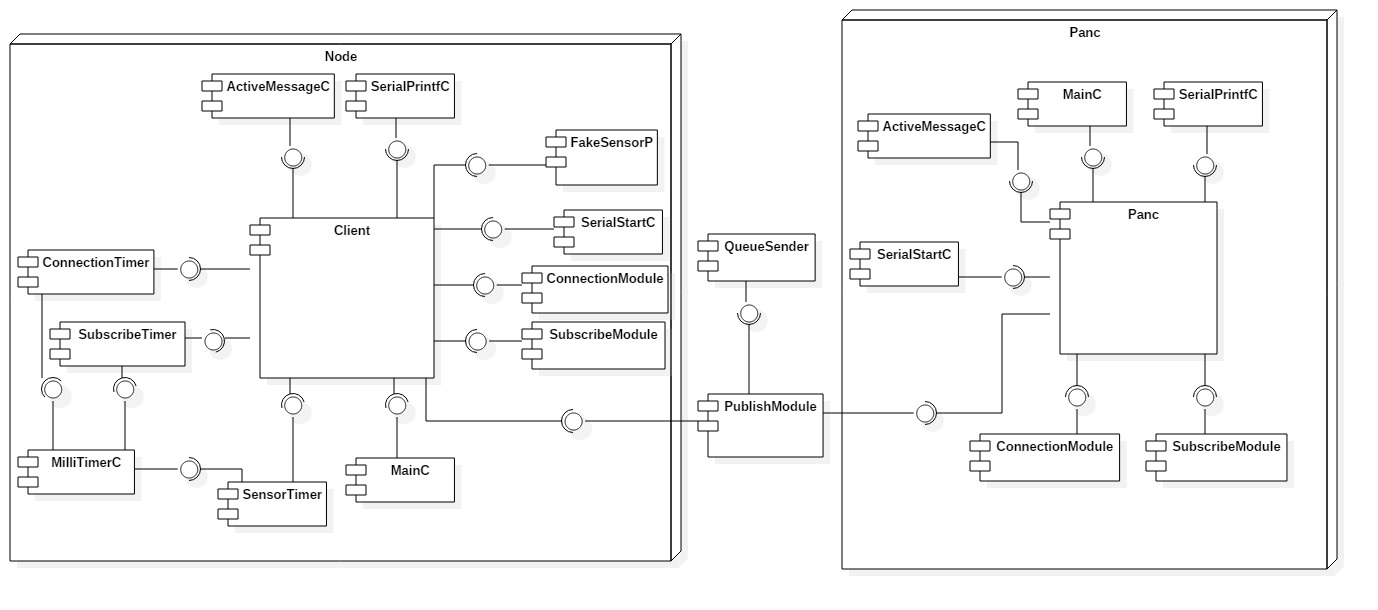
\includegraphics[scale=0.35]{ComponentDiagram}
\end{figure}
\begin{figure}[h]
\caption{Sequence diagram of \emph{Publish} procedure.}
\centering
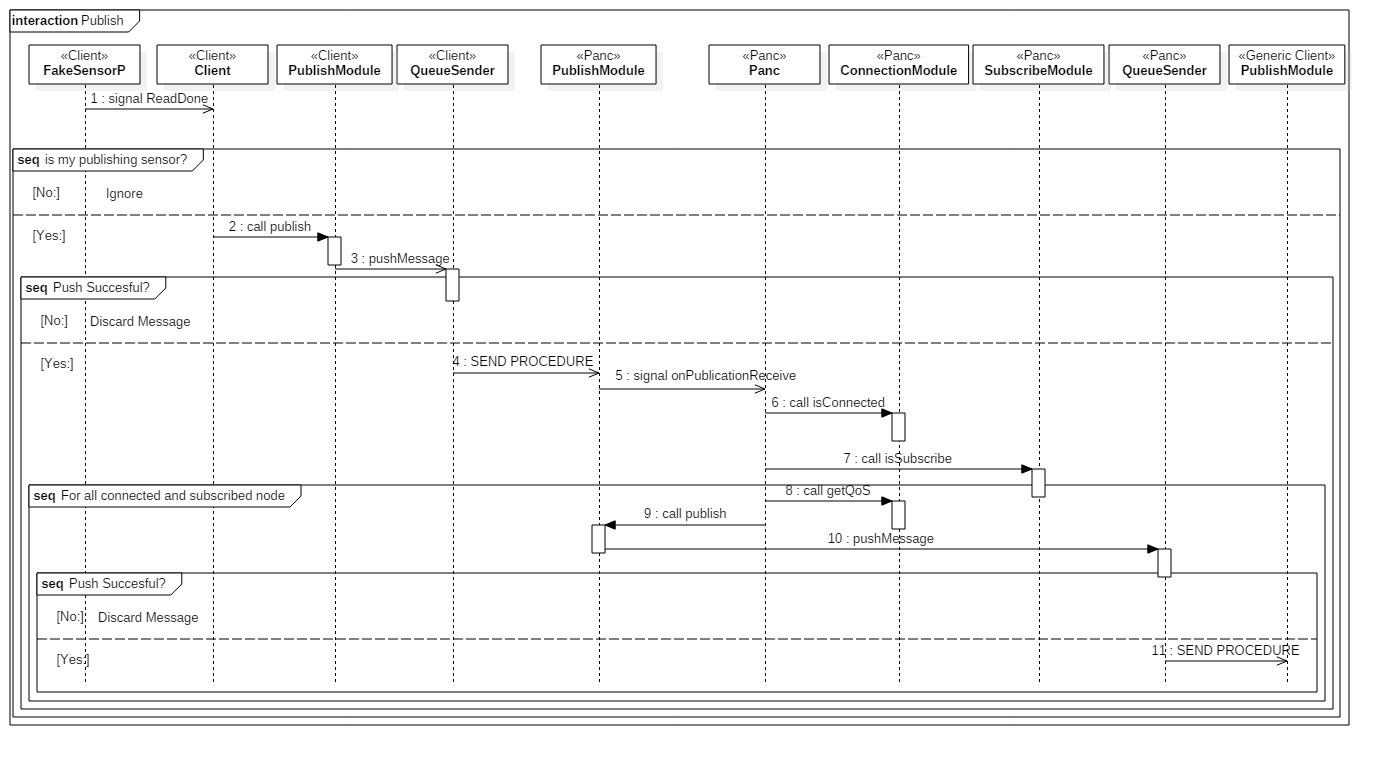
\includegraphics[scale=0.35]{Publish}
\end{figure}




\end{document}